\section{Introduction}
The design phase of the web application, focused on using emotion recognition to generate music therapy playlists, represents a bridge from theoretical concepts to a operational system.
The varied design approaches that were used to develop an application with a solid technical framework and user-friendly interface are covered in this section.
\\
\indent The core aspect of the application is how it uses captured frame analysis to determine a user's emotional state by utilizing \gls{fer} technology.
This sense of emotional then guided the creation of customized music playlists, fusing the advanced machine learning techniques with the restorative properties of music to provide a unique advantageous user experience.
\\
\indent This project uses diagrams such as block diagram, use case diagram, sequence diagram and etc., where each focusing on a different aspect of the architecture and functionality of the system.
Futhermore, this section delves into the visual and functional components of the application's user interface as illustrated by the Logo Design and Interface Design.
The logo, as the visual cornerstone of the application's brand identify, have been thoughtfully designed to improve application usability and user engagement.
\\
\indent Additionally, the \gls{ml} model architecture design, which describes the underlying algorithms and data processing methods used in \gls{fer}, is also discussed in this section.
This discussion covers the model's validation, training, and integration into the broader application ecosystem to ensure accurate emotional analysis.
\\
\indent All of these components provide a thorough explanation of the system's design, addressing structural, behavioral, and aesthetic factors from the abstract to the concrete.

\section{Web Application}
\subsection{UML Diagrams}
\subsubsection{Block Diagram}
Block diagram present a high-level overview of the system's architecture, highlighting the major components and their interactions. \citep{freeman_block}
This offers insights into the overall system design and its flow.
\begin{figure}[!ht]
    \centering
    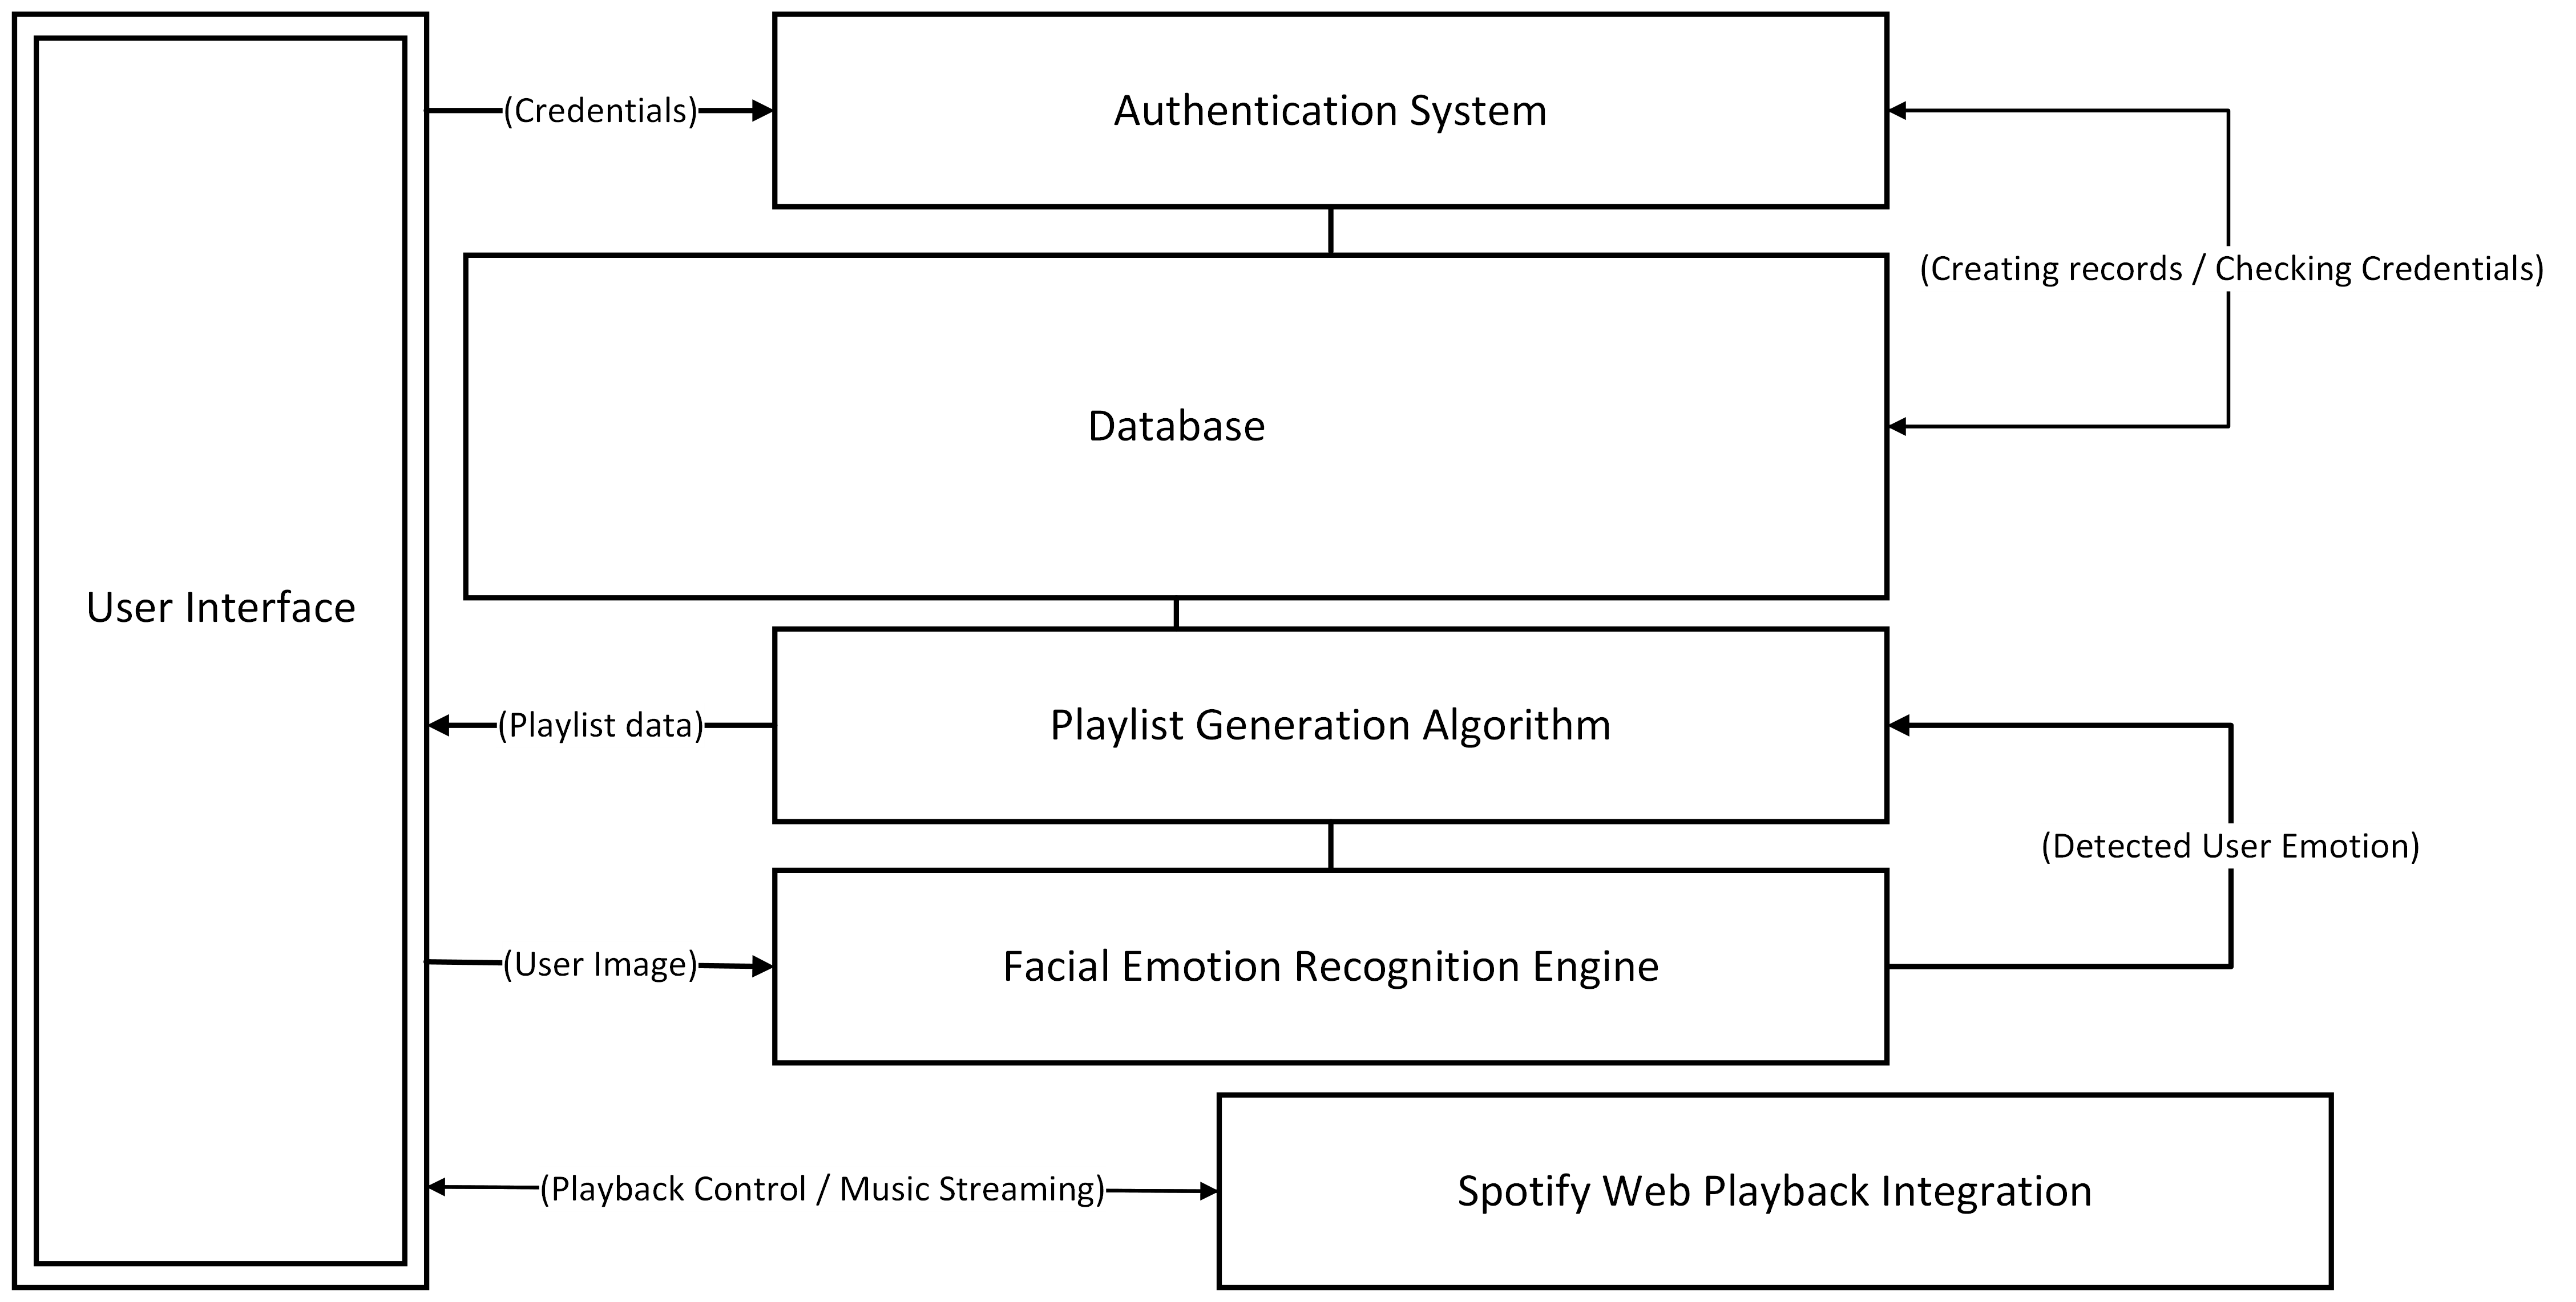
\includegraphics[width=12cm]{Images/block.png}
    \caption{Block Diagram}
    \label{fig:block}
\end{figure}
\\
\indent From Figure \ref{fig:block}, there are different components and each component has its own responsibilities to enable \gls{fer} and playlist generation for music therapy.
\gls{ui} is the gateway through which users interact with the application.
It captures user inputs such as credentials for the authentication process, frames for emotion recognition, and user actions for music playback controls.
\\
\indent Authentication System manages user identity verification and access control.
When user provides credentials, either username or email, and password to this component, it will validates them against stored data in the database. 
Upon successful validation, users can access the full functionality of the services.
This component also handles account creation, where new user details are stored securely in the database.
\\
\indent Database stores and manages all persistent data, including user credentials, profile information, and any data pertinent to playlist generation processes.
It ensures data integrity and provides efficient access for other components.
\gls{fer} Engine utilizes advanced algorithms and machine learning models.
This engine analyses captured frame, which contains user's facial expression, to detect emotional states.
The result of this analysis is then used to tailor the music playlist to the user's current emotional needs.
\\
\indent Playlist Generation Algorithm takes the detected emotion from the \gls{fer} Engine and constructs a playlist that suits the identified mood and therapeutic requirements.
It queries a database of songs, which stored internally, to select appropriate tracks.
Then, Spotify Web Playback Integration acts as the music service interface. 
This component is responsible for fetching the actual music tracks from Spotify and controlling the playback within the application, such as playing, pausing, and etc. based on user input through the \gls{ui}.
\\
\indent This diagram simplifies the conceptual understanding of the system and forms the architectural backbone of the application.
It also outlines how user actions translate into system responses and result in a music therapy experience.
\\
\subsubsection{Use Case Diagram}
Use Case diagram is a visual representation of the system's functionalities and the interactions that different types of users have with these functionalities. \citep{ibm_2021_usecase}
\begin{figure}[!ht]
    \centering
    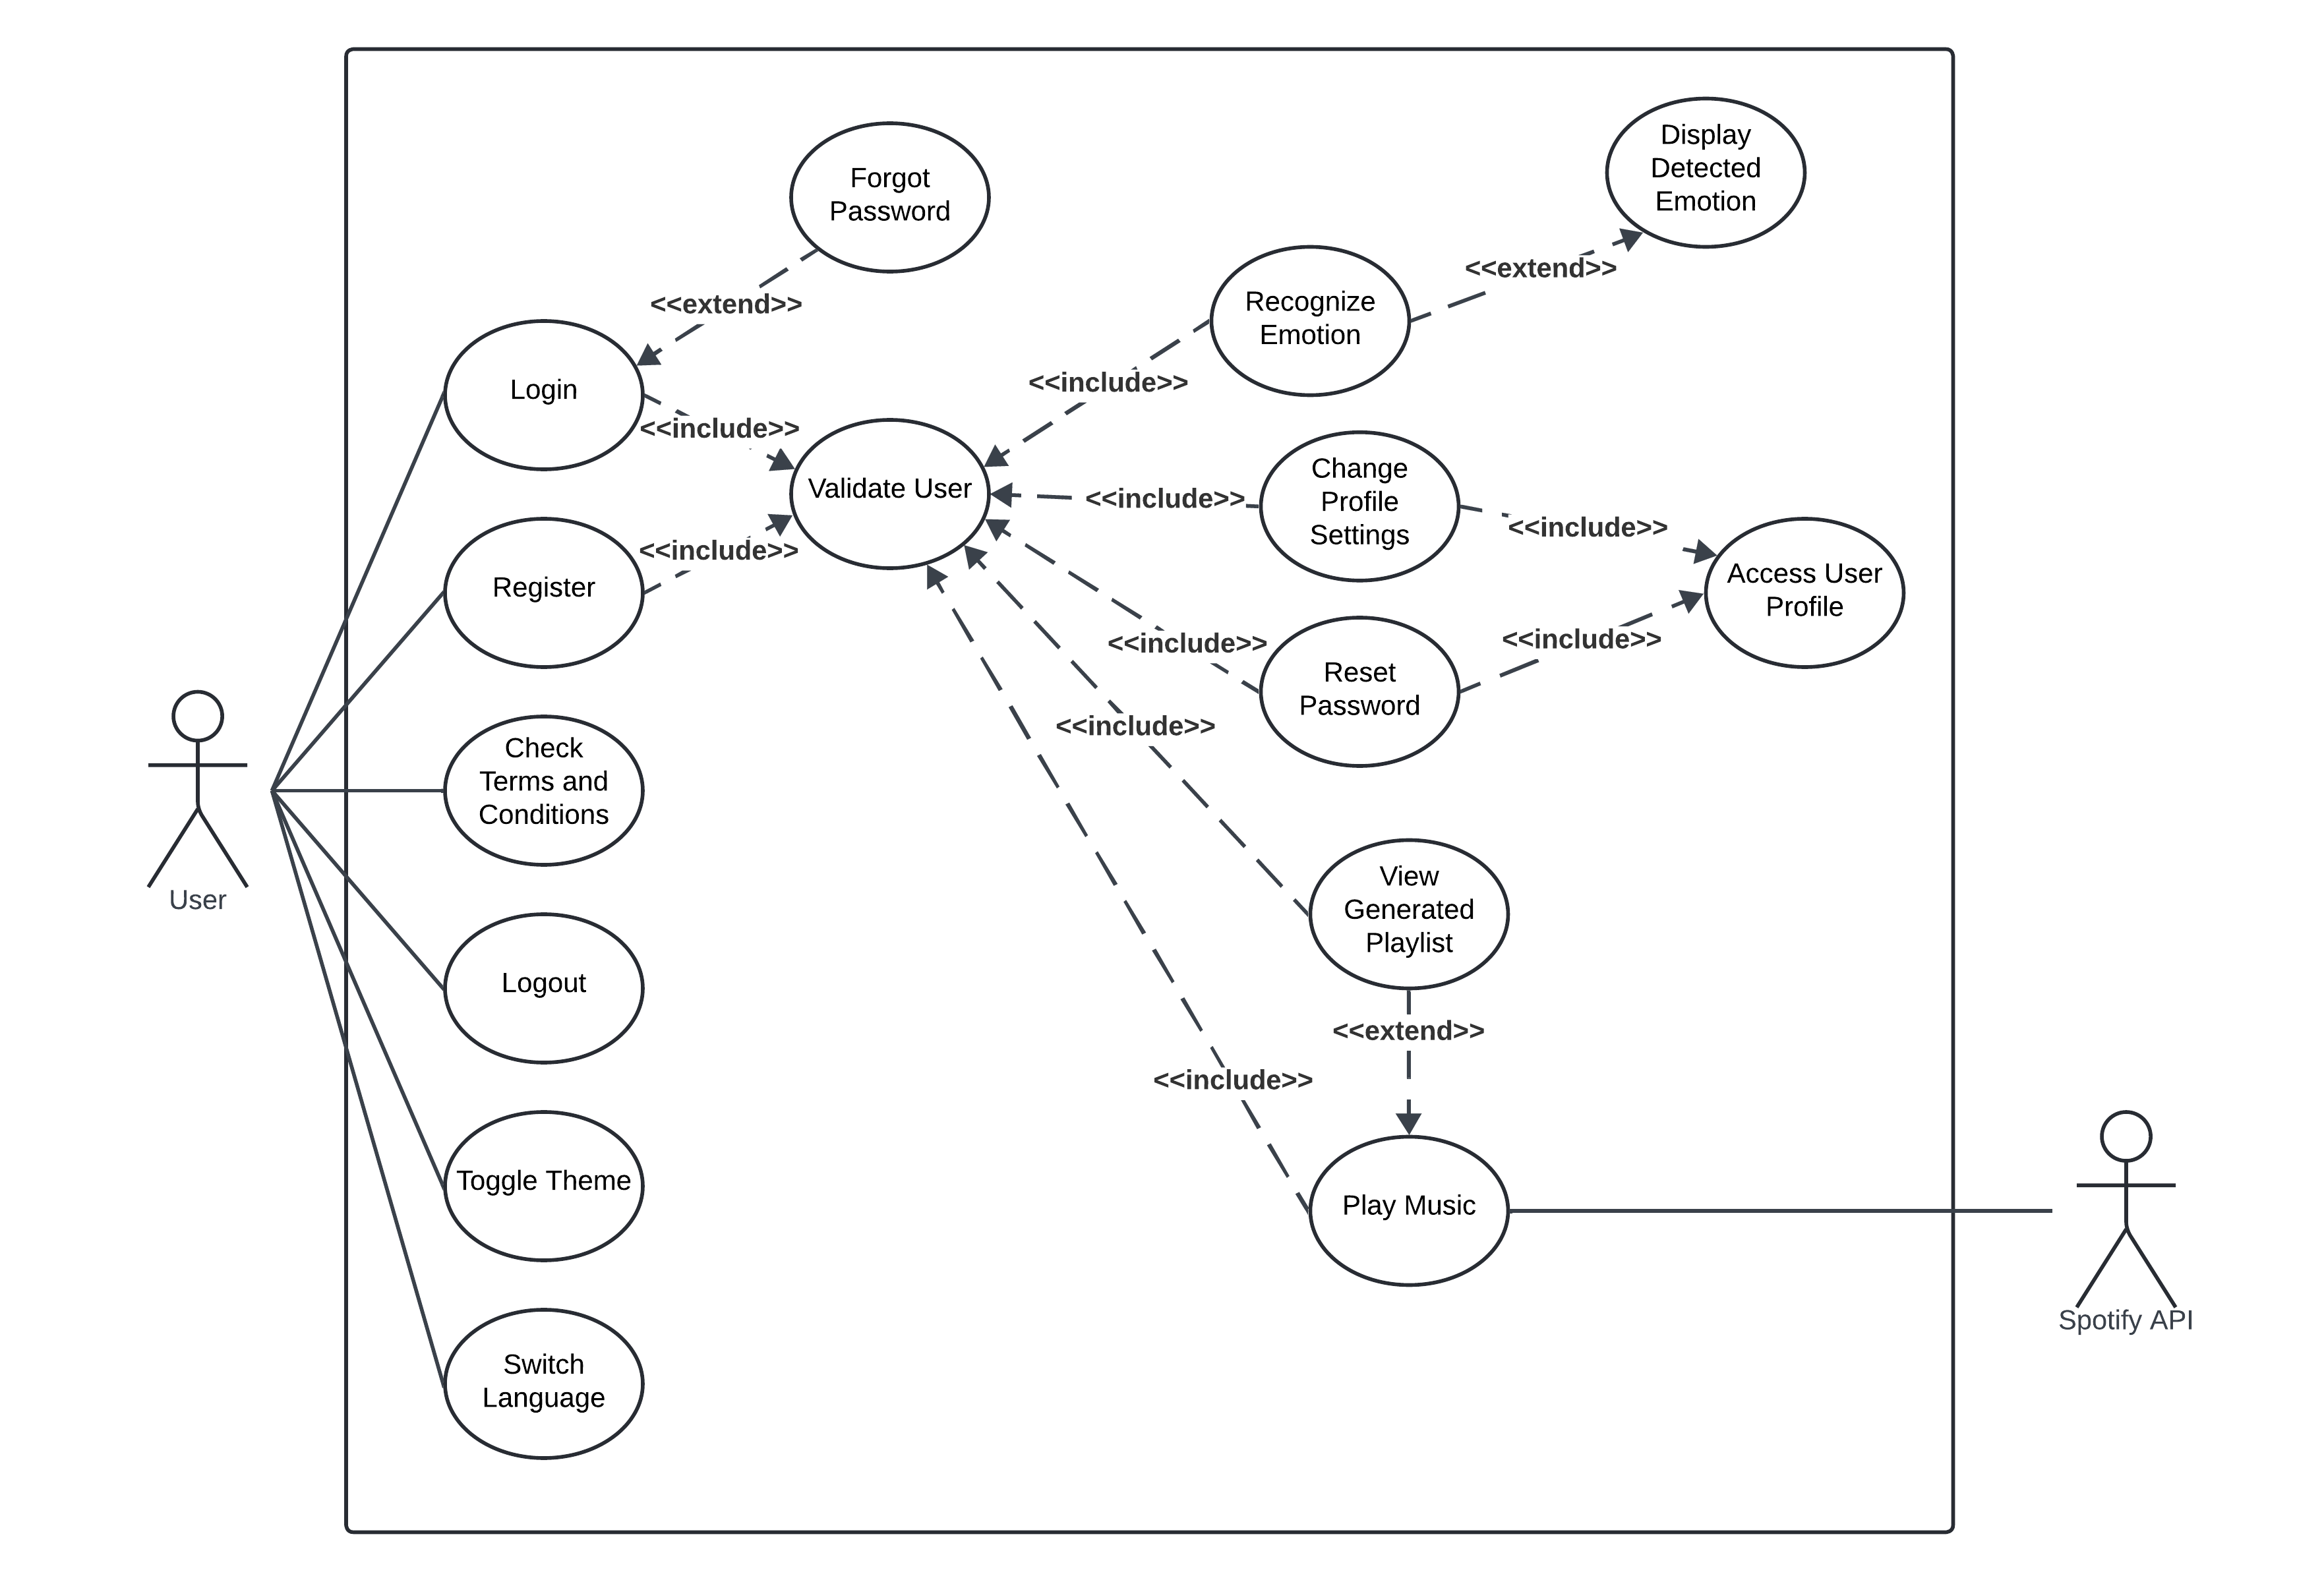
\includegraphics[width=14cm]{Images/usecase.png}
    \caption{Use Case Diagram}
    \label{fig:usecase}
\end{figure}
\\
\indent In Figure \ref{fig:usecase}, there are two actors, `User' and the `Spotify API'.
The `User' represents any individual who interacts with the application for its services.
The `Spotify API' acts as an external system that the application communicates with to stream music.
\\
\indent The use case diagram delineates the extent of the application's capability from the `User' point of view by illustrating the user interactions.
This helps to understand what the system does, but not how it does it, thus separating the `what' from the `how' in system functionalities.
When a use case incorporates another's behavior or expands the behavior under some circumstances, it is represented by dashed lines with arrows labelled `includes' and `extends.'
For example, several use cases in the application such as `Recognize Emotion', `Change Profile Settings', and `Play Music', require the `User' to be authenticated.
This precondition is captured in the `Validate User' use case, which is included in these use cases to ensure that the `User' is logged in before granting access to the services.
\\
\subsubsection{Sequence Diagrams}
Sequence diagrams provide an illustrative view of how various components of a system work together ot accomplish a process, acting as blueprints of interaction across time.\citep{bell_2004_explore}
They are especially helpful in understanding the flow of messages and actions between objects in response to software system events.
\begin{figure}[!ht]
    \centering
    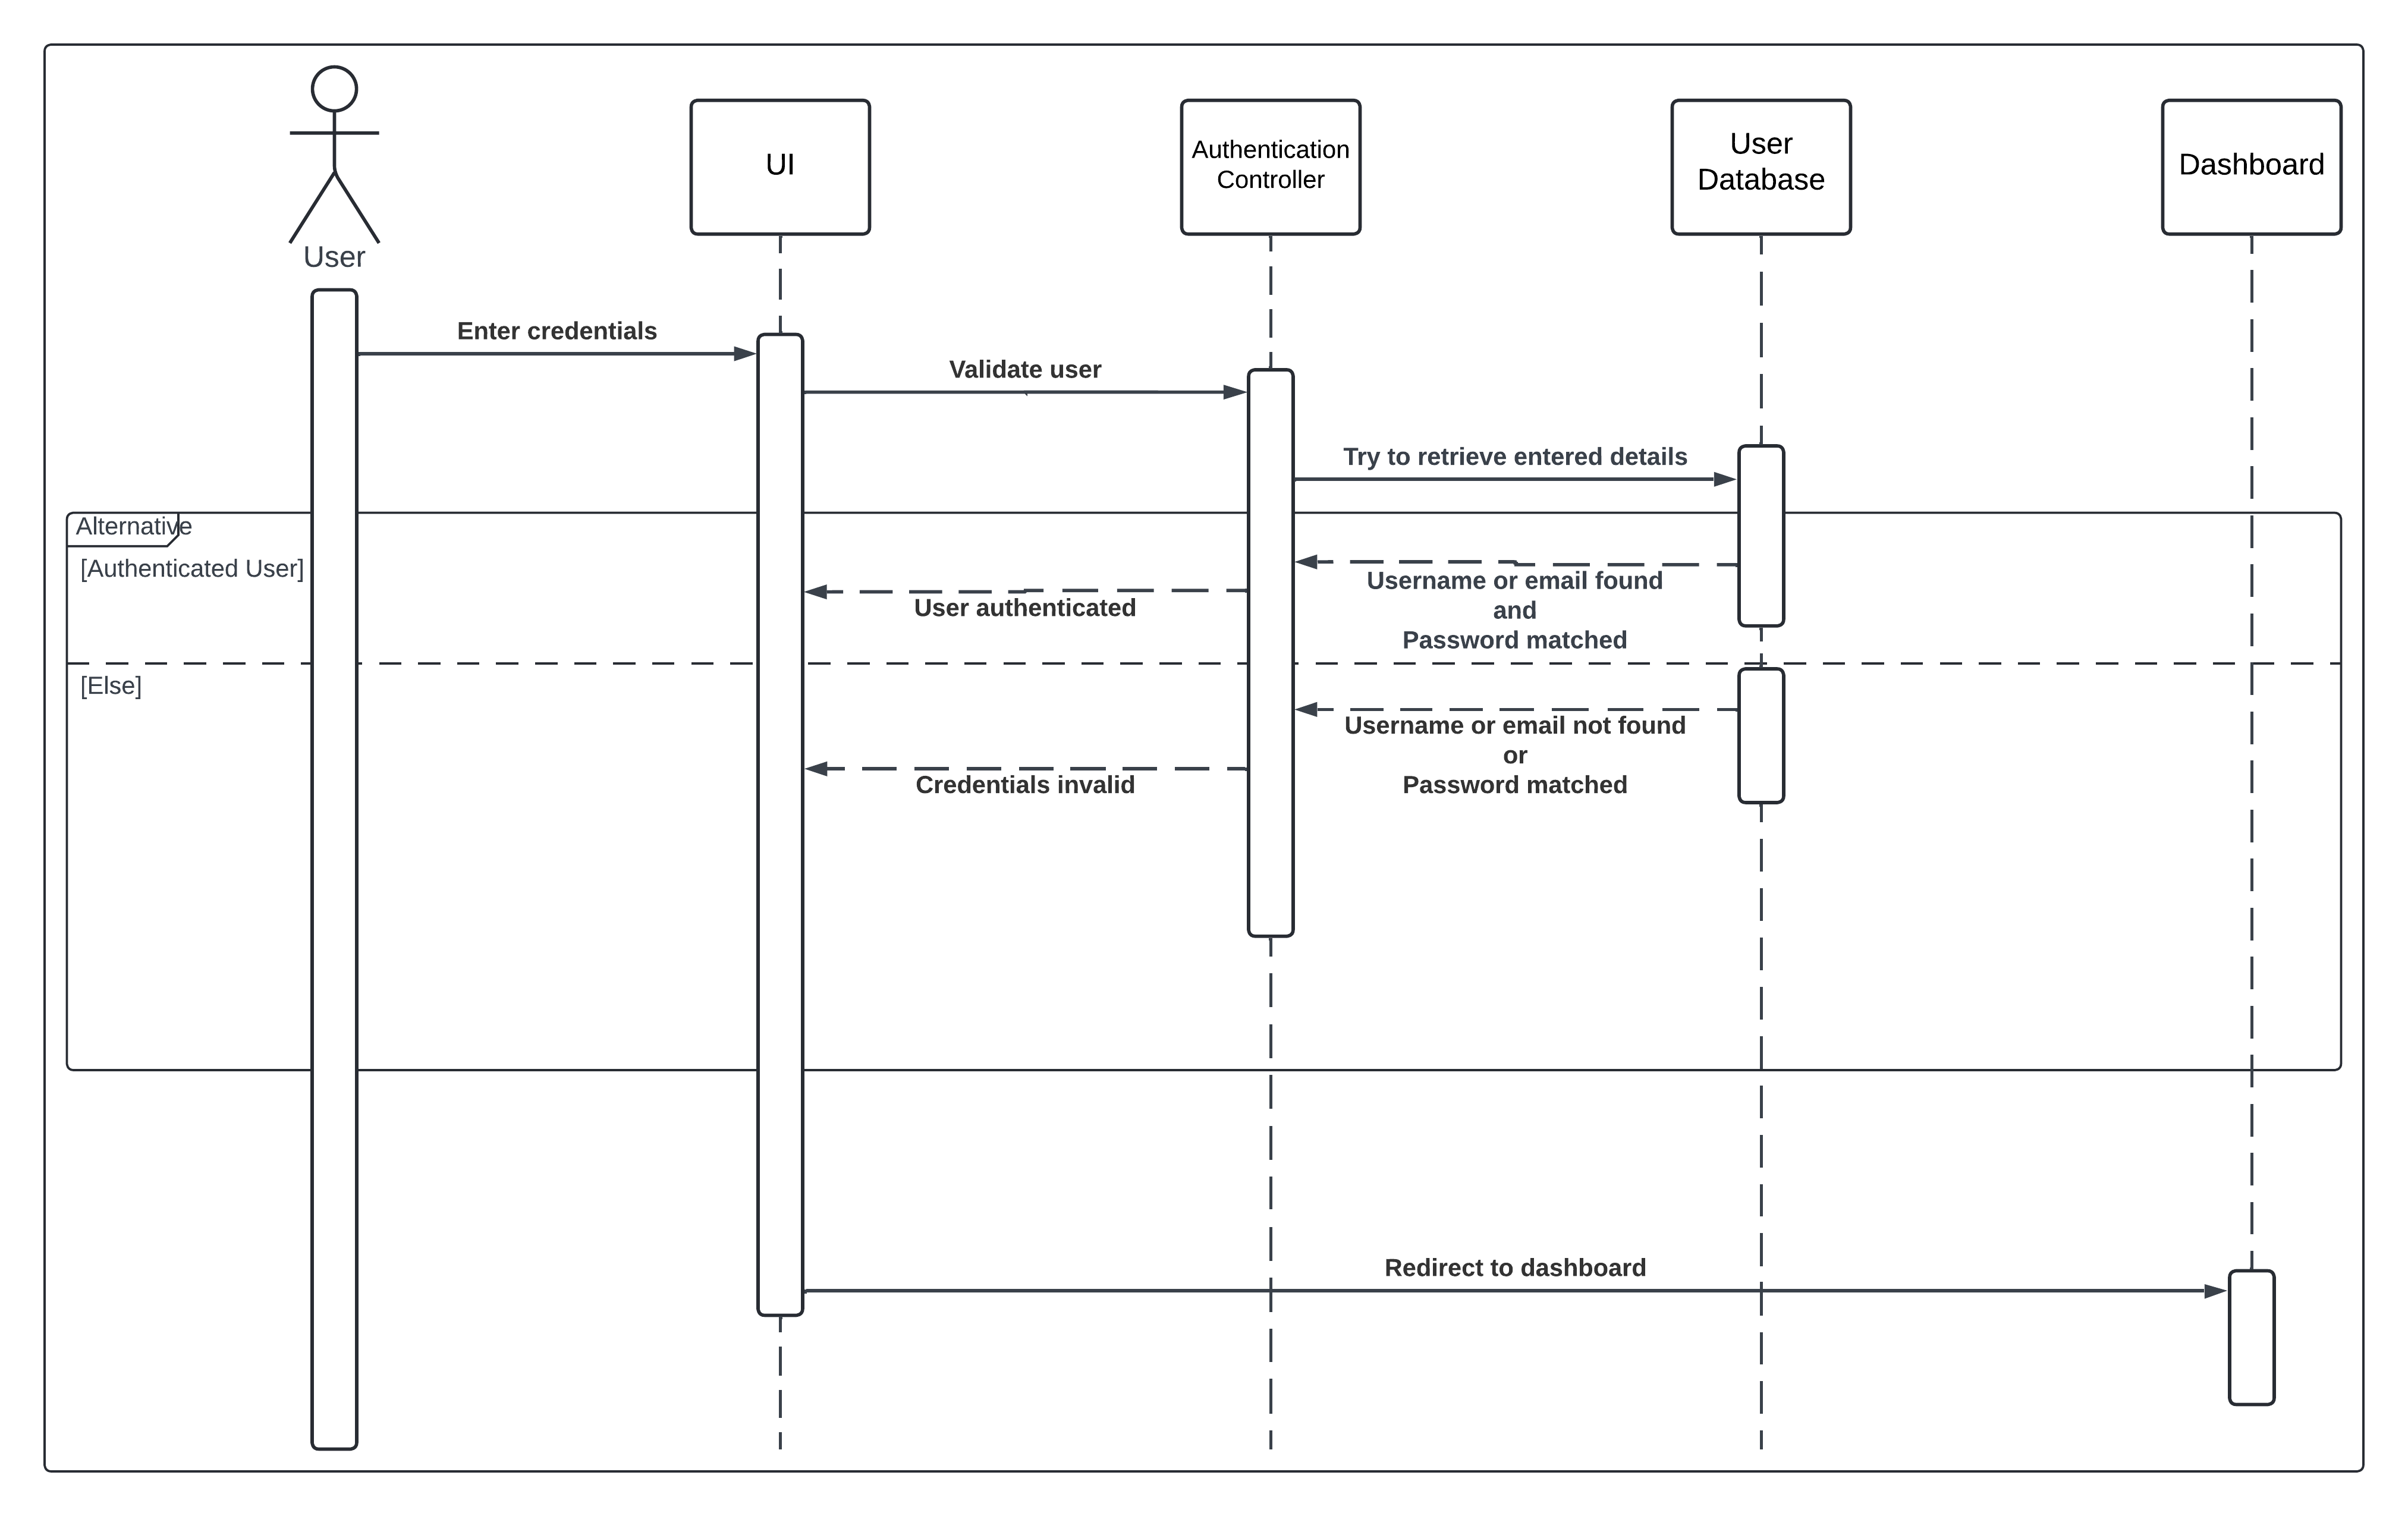
\includegraphics[width=14cm]{Images/login-sequence.png}
    \caption{Login Sequence Diagram}
    \label{fig:login-sequence}
\end{figure}
\begin{figure}[!ht]
    \centering
    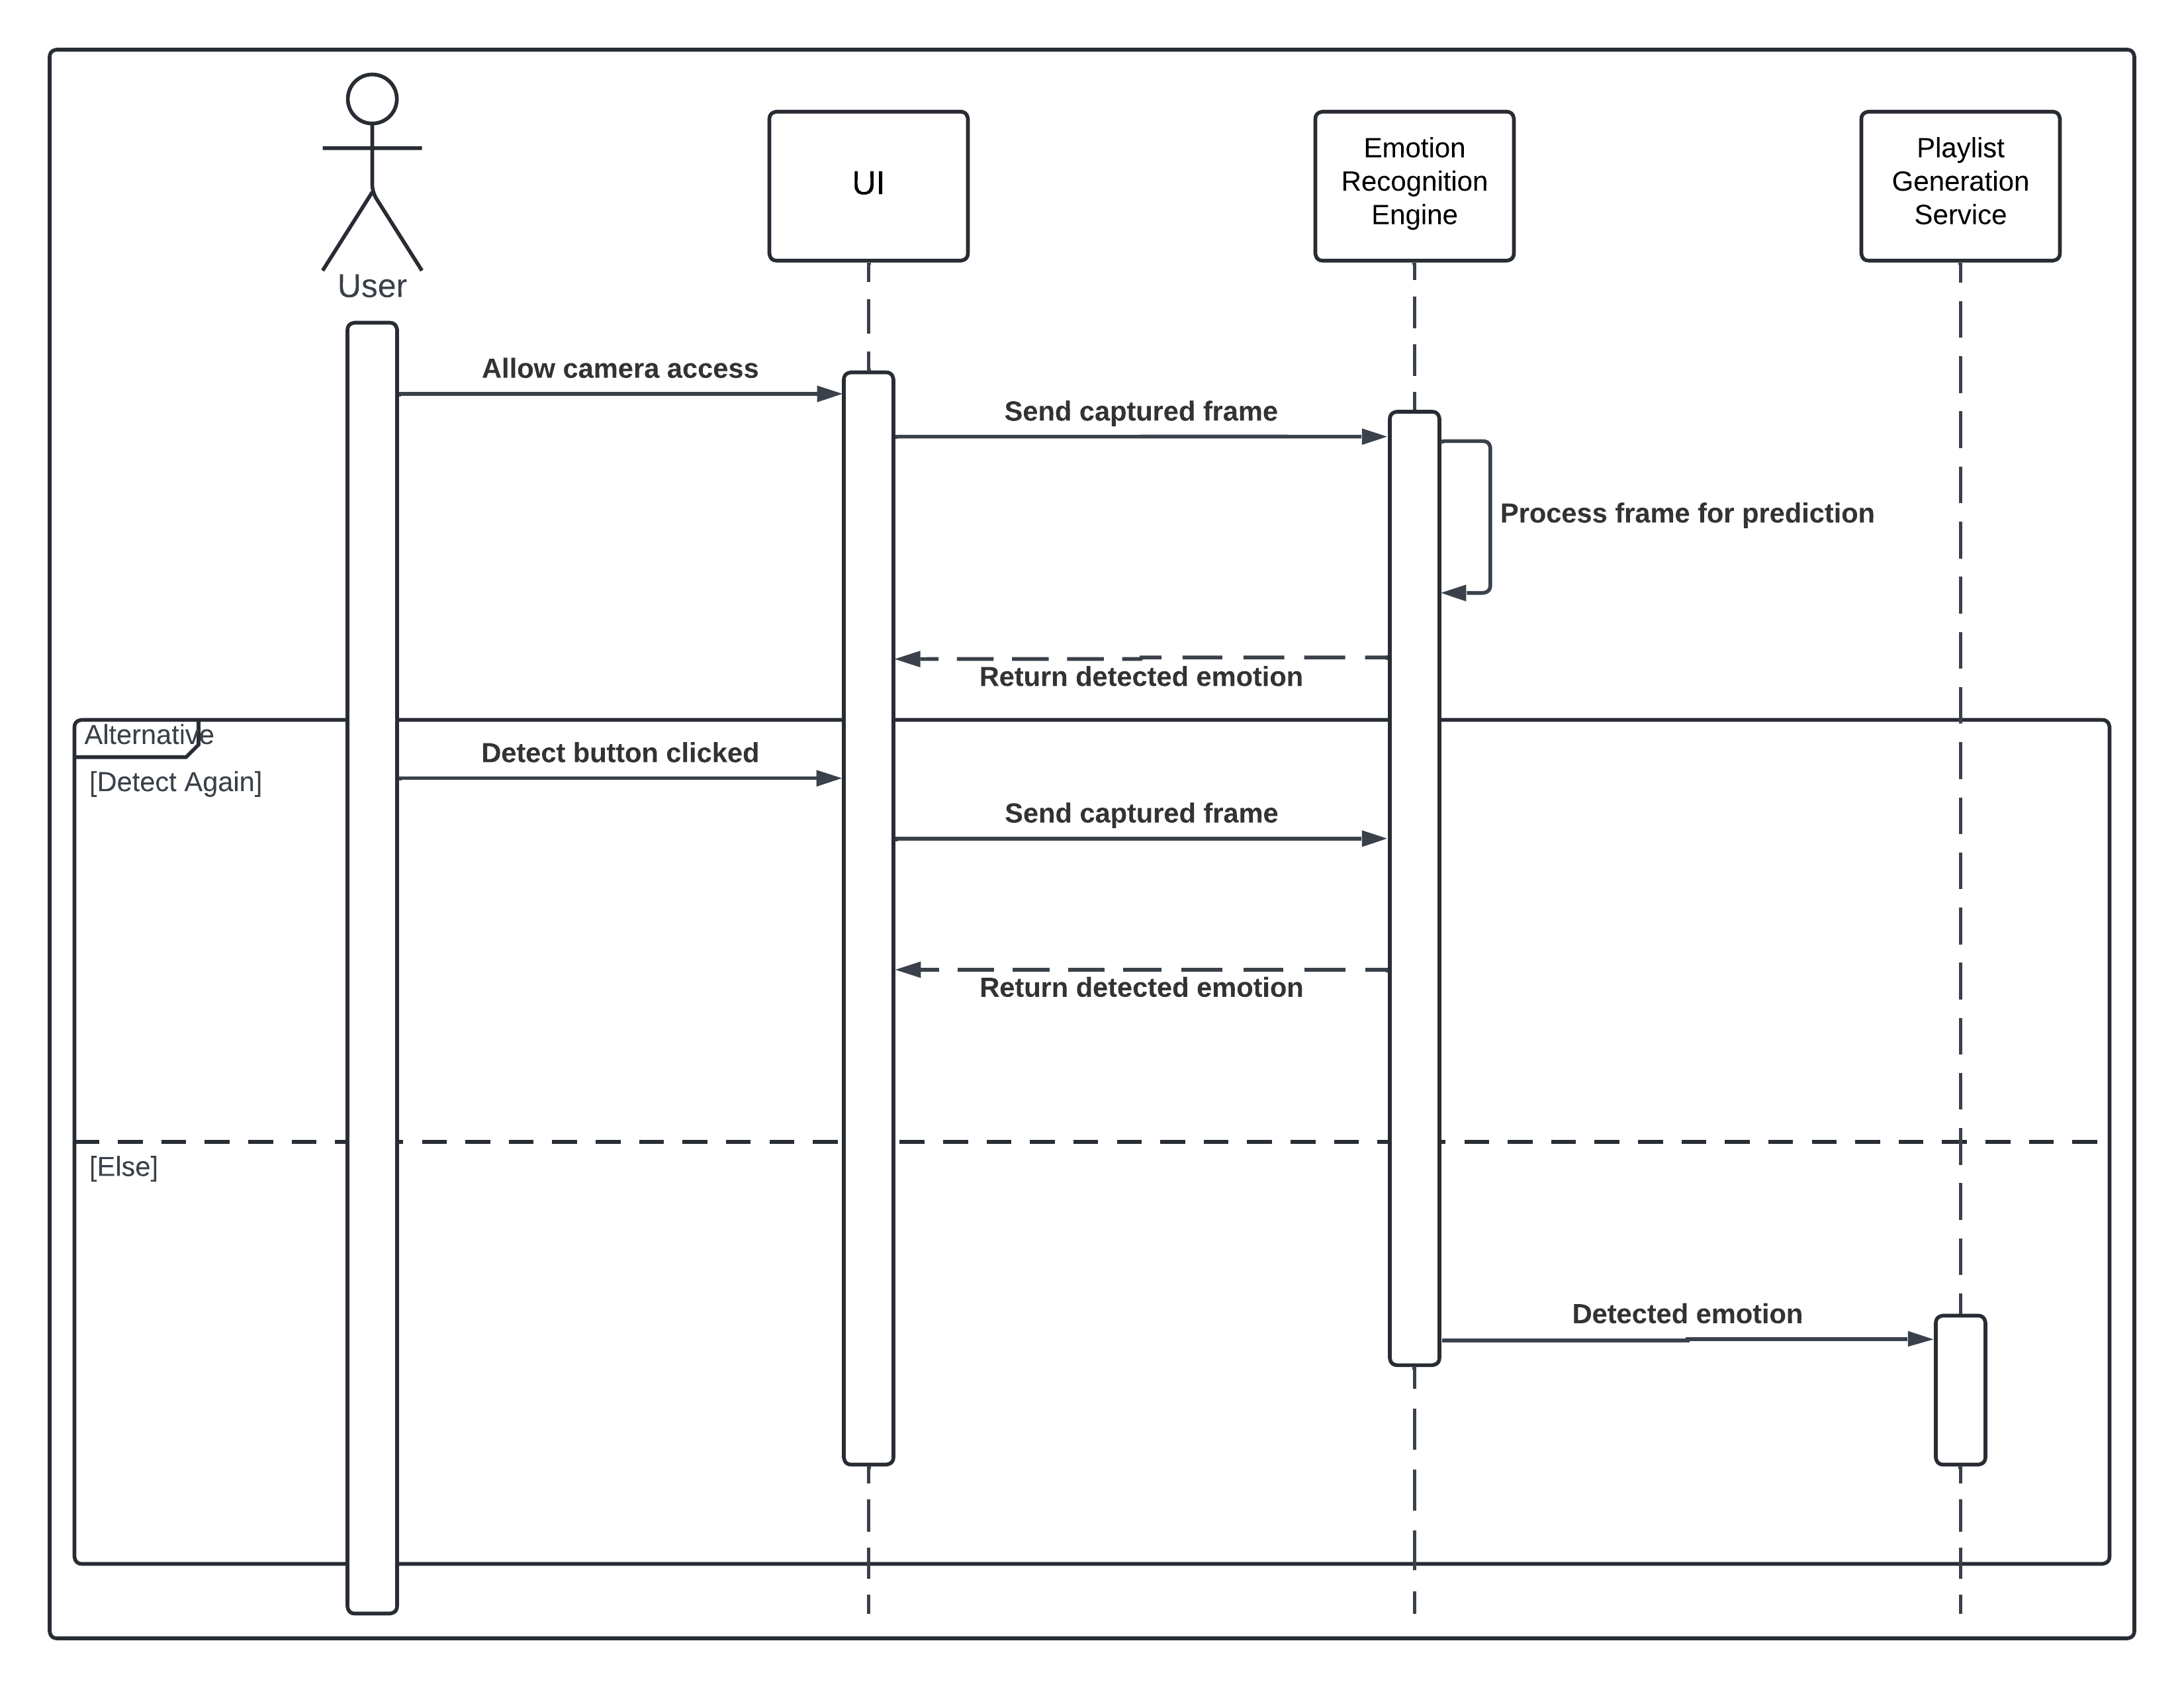
\includegraphics[width=14cm]{Images/fer-sequence.png}
    \caption{Emotion Recognition Sequence Diagram}
    \label{fig:fer-sequence}
\end{figure}
\begin{figure}[!ht]
    \centering
    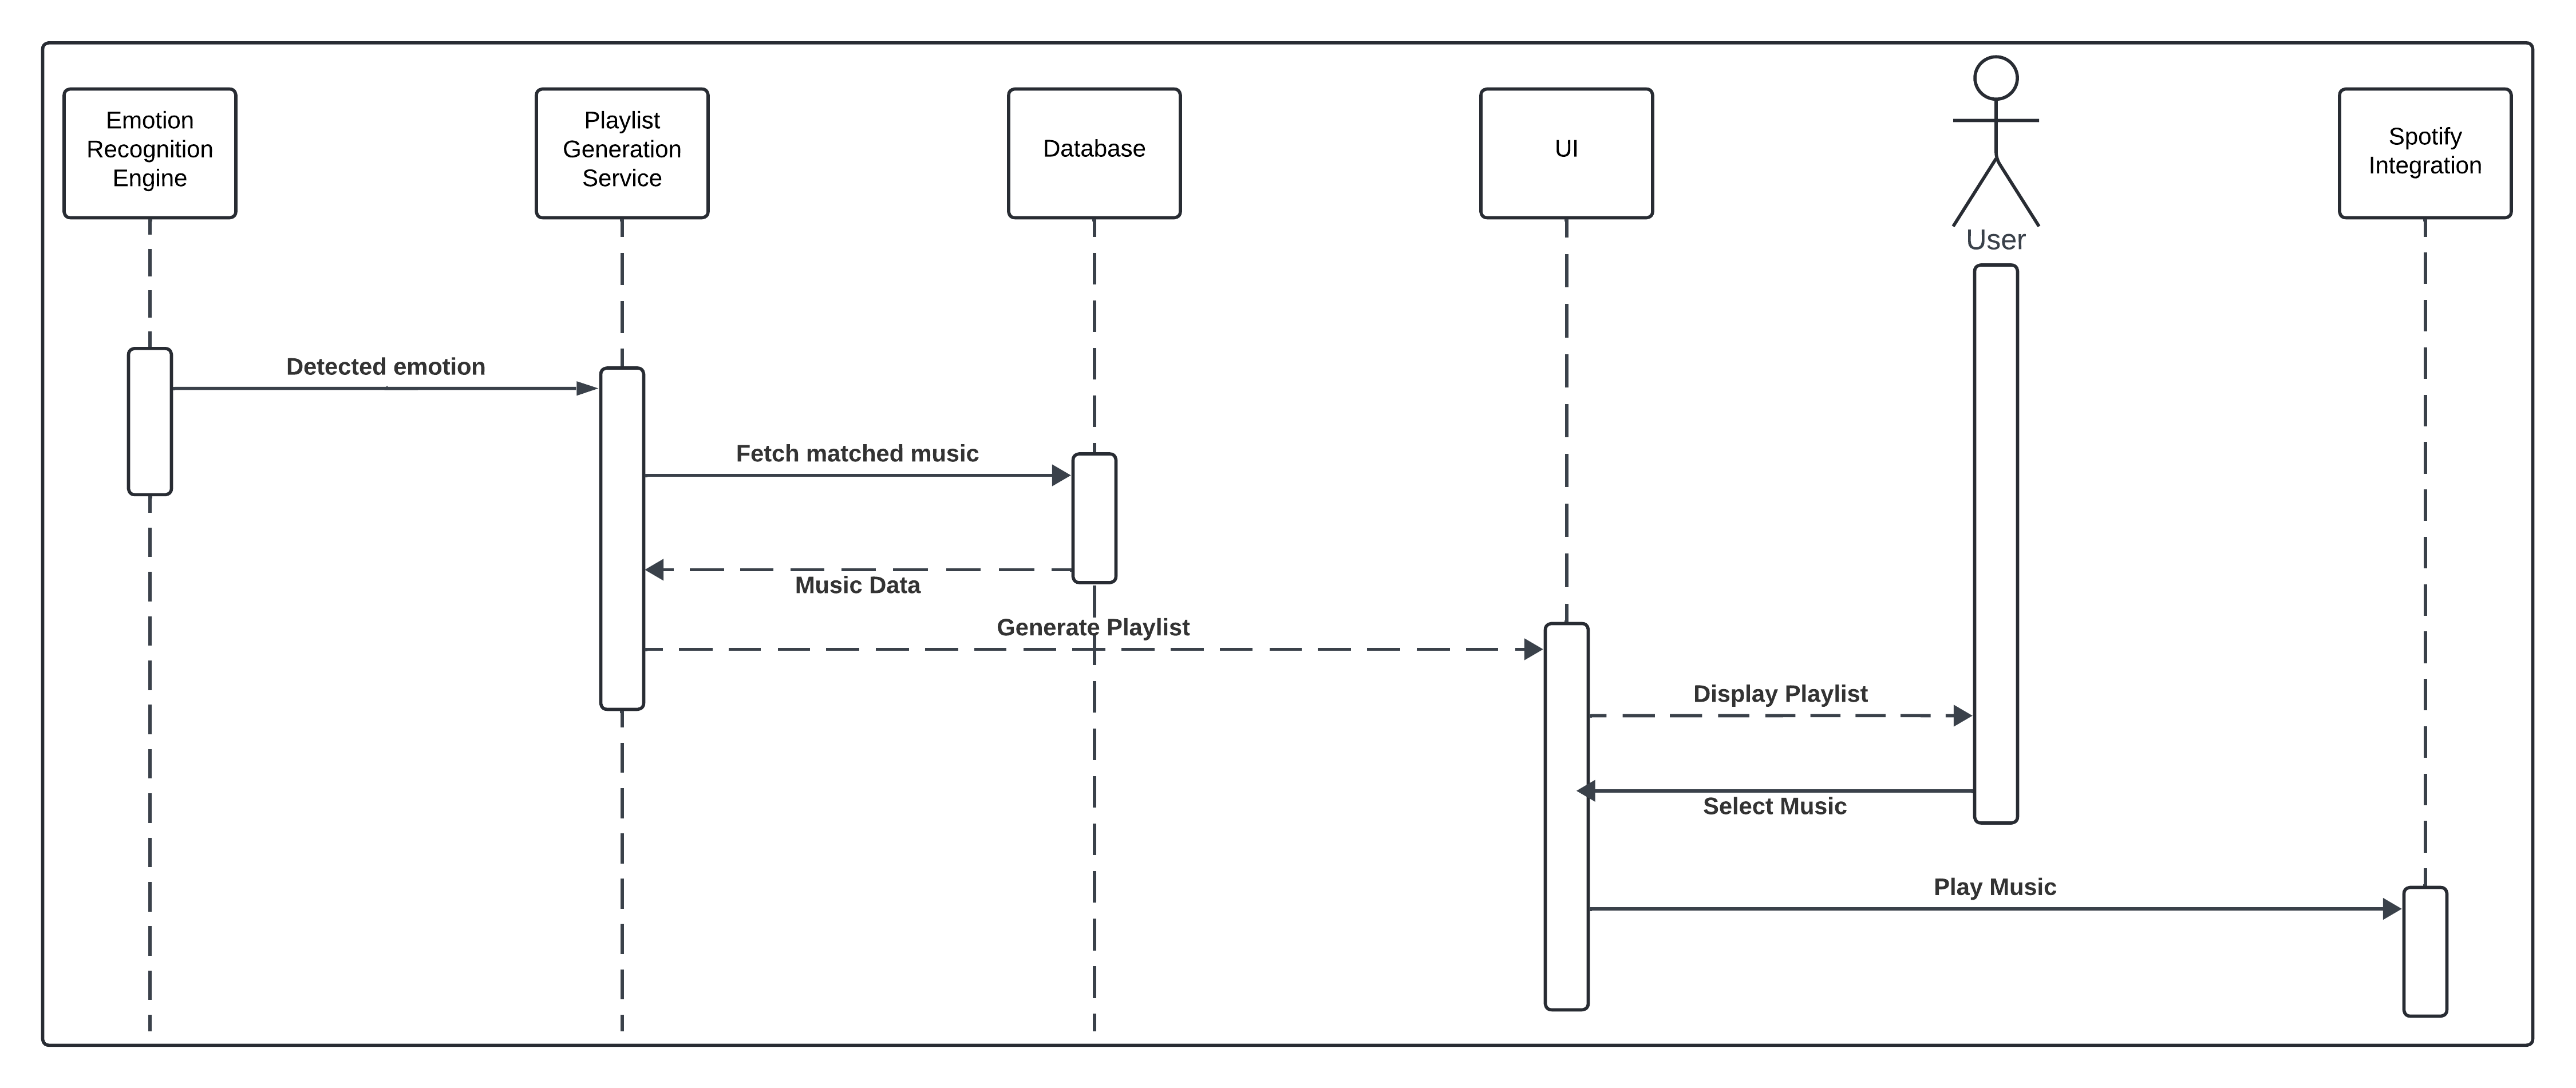
\includegraphics[width=14cm]{Images/playlist-sequence.png}
    \caption{Playlist Generation Sequence Diagram}
    \label{fig:playlist-sequence}
\end{figure}
\\
\indent Figure \ref{fig:fer-sequence} presents the series of interactions that commence with capturing a user's facial expression and terminates when the system identifies the user's emotional state.
The sequence is outlined from the user interface to the backend services, where the input is processed by the `Emotion Recognition Engine' to identify emotion. 
The detected emotion will then influence the music playlist generation. 
\\
\indent Figure \ref{fig:playlist-sequence} shows how the service uses the detected emotion from Figure \ref{fig:fer-sequence} to choose and assemble a series of songs into a coherent playlist.
From retrieving suitable songs based on the emotional analysis to returning the playlist to the user for playback through Spotify Web Playback service, it demonstrates the cooperation between the system's components.
\\
\subsubsection{Flowchart}
Flowchart represent the process of a system, the decisions that need to be made, and the flow of control from one step to the next.
Troubleshooting and system design are made considerably easier with the aid of flowchart as they make the sequential phase and logic paths in complicated processes visible. \citep{lucidchart_2019_what}
\begin{figure}[!ht]
    \centering
    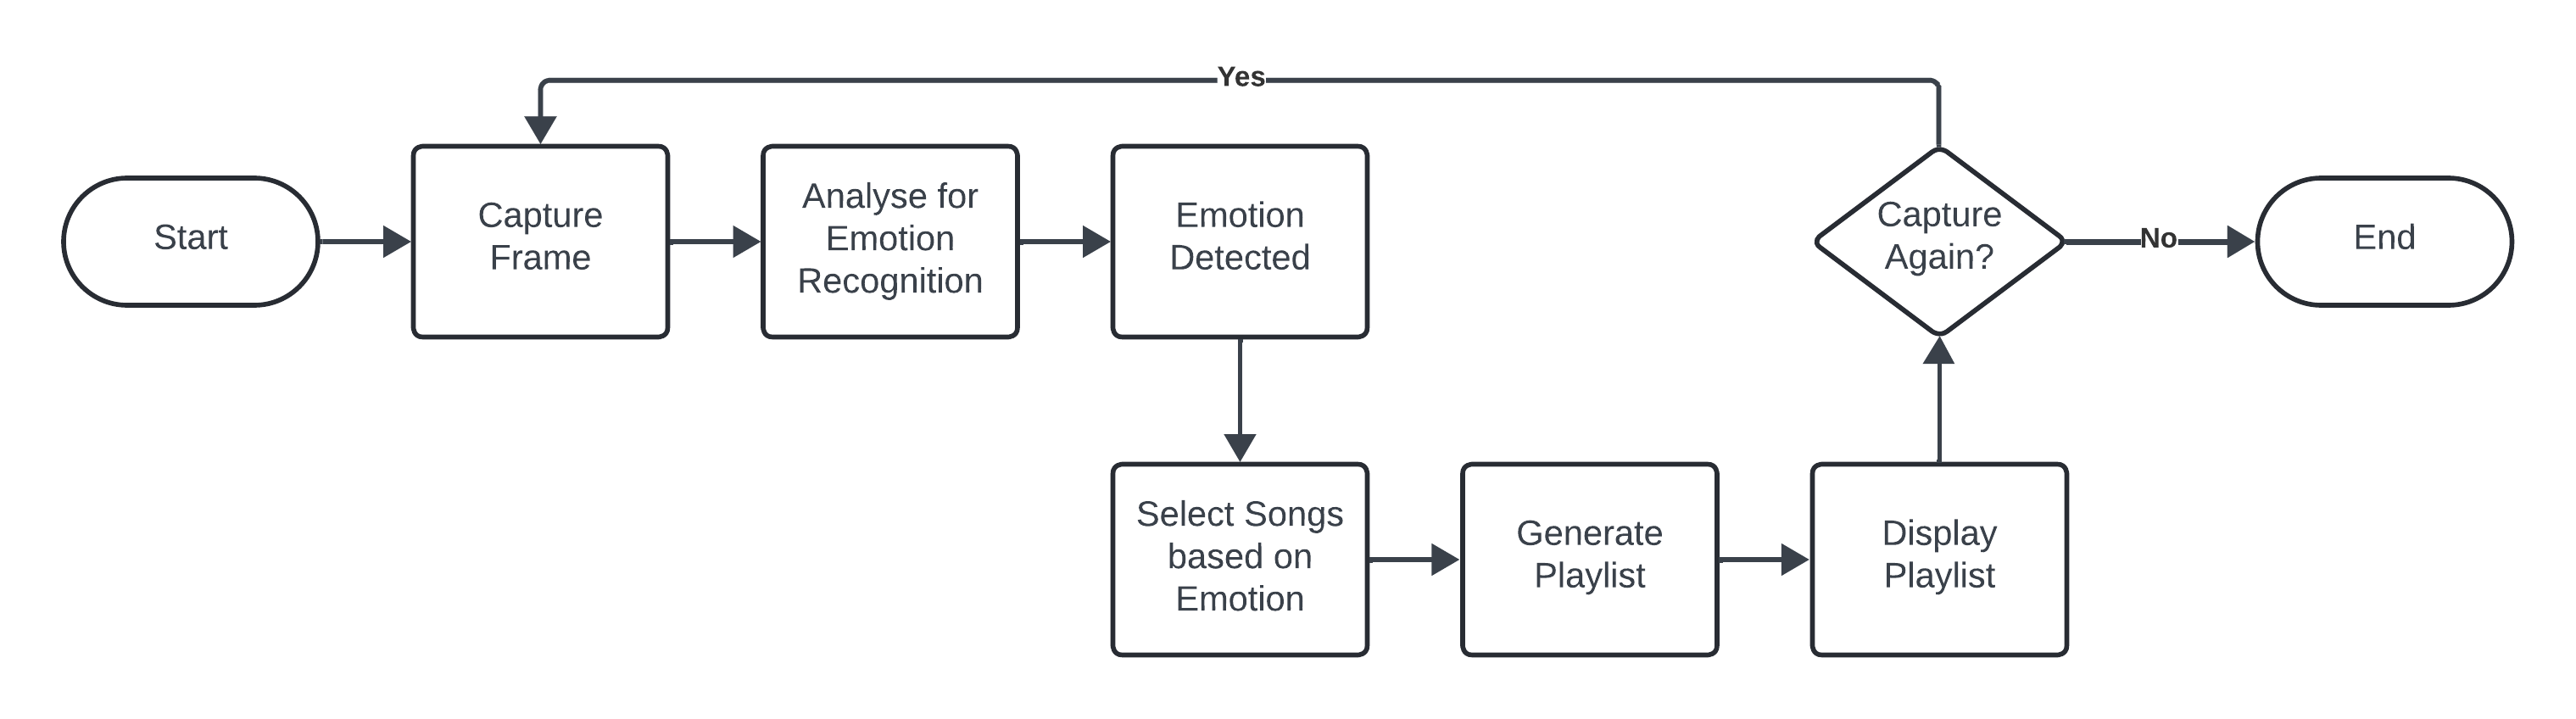
\includegraphics[width=14cm]{Images/flowchart.png}
    \caption{Flowchart For Emotion Recognition and Playlist Generation}
    \label{fig:flowchart-fer-pg}
\end{figure}
\\
\indent Figure \ref{fig:flowchart-fer-pg} shows the steps taken from the moment a user engages with the feature to capture their emotional state to the point where the system recognizes and outputs the detected emotion.
Following the \gls{fer} phase, the identified emotion is then used to select suitable music, creating playlist and presenting it to the user. 
\\
\subsubsection{Entity-relationship Diagram}
\gls{erd} is a structured representation of the data entities within the web application and the interconnections between them. 
This illustration outlines the database schema, which is foundational for storing, retrieving, and managing data that the application operates upon.
\begin{figure}[!ht]
    \centering
    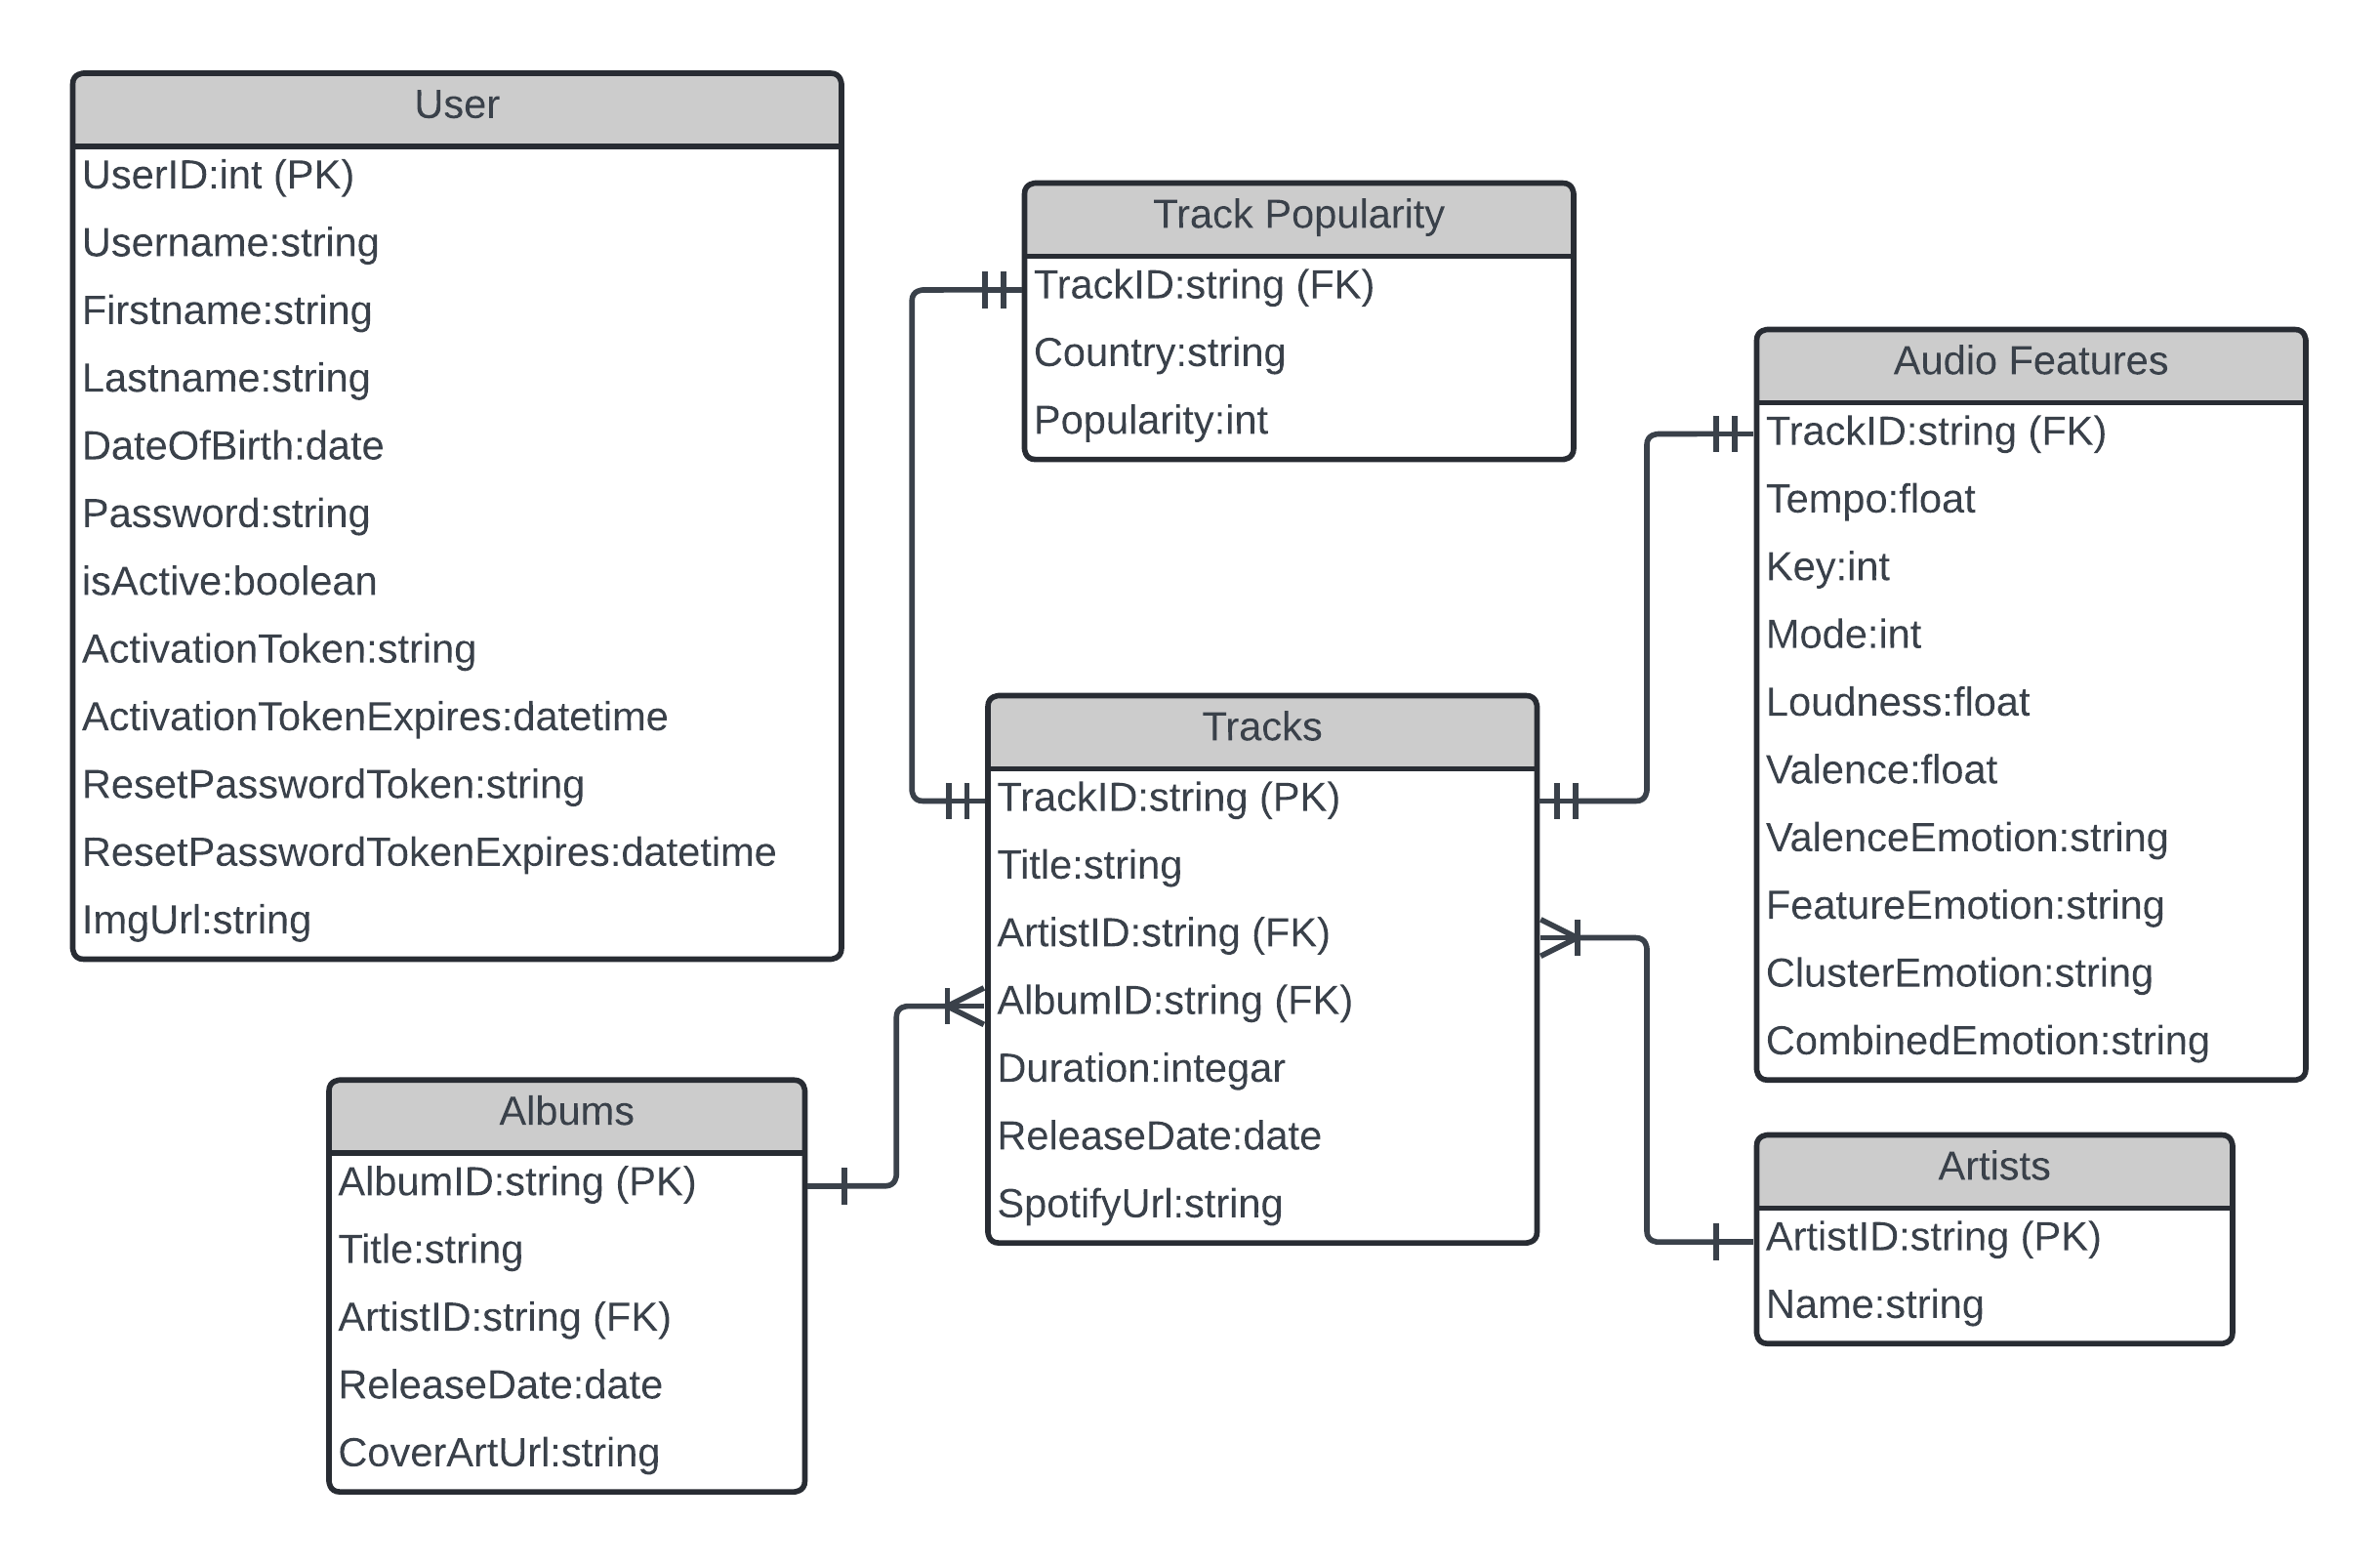
\includegraphics[width=14cm]{Images/erd.png}
    \caption{Entity-relationship Diagram}
    \label{fig:erd}
\end{figure}
\\
\indent Figure \ref{fig:erd} presents the \gls{erd} for the application.
`User' representing the application's users, containing `UserID', `Username' and other personal details which could be modified in `User Settings Page' (Figure \ref{fig:usr-settings}).
`Albums', `Tracks', `Audio Features', `Track Popularity', and `Artists' are entities that stored music data from song title to information such as its tempo, its loudness and other audio features.
\\
\indent The relationship between entities are defined by \gls{pk} and \gls{fk}, enforcing referential integrity within the database.
For example, a one-to-many relationship from `Artists' to `Tracks' indicates that one artist can have multiple tracks, whereas a one-to-one relationship between `Tracks' and `Audio Features' indicates that each track has its own unique features.
\\
\subsection{Logo Design}
Figure \ref{subfig:light-logo} and Figure \ref{subfig:dark-logo} is made up of stylized waves that reference the soothing rhythms of ocean waves while also visualizing the representation of an audio signal.
This duality shows the fundamental purpose of the application, using the ability of music to evoke and influence emotions, providing a calming and therapeutic user experience.
\begin{figure}[h!]
    \centering
    \subfloat[\centering Logo \label{subfig:light-logo}]{{
\includegraphics[width=3cm]{Images/dark.png}}}%
    \qquad
    \subfloat[\centering Banner\label{subfig:light-banner}]{{
\includegraphics[width=7cm]{Images/dark-banner.png}}}%
    \vspace{0.5cm}
    \\
    \caption{Light Theme Logo}
\end{figure}
\begin{figure}[h!]
    \centering
    \makebox[\textwidth]{
        \begin{minipage}{14cm} 
            \begin{mdframed}[backgroundcolor=gray!70]
                \centering
                \subfloat[\centering Logo \label{subfig:dark-logo}]{{
\includegraphics[width=3cm]{Images/light.png}}}%
                \qquad
                \subfloat[\centering Banner\label{subfig:dark-banner}]{{
\includegraphics[width=7cm]{Images/light-banner.png}}}%
            \end{mdframed}
        \end{minipage}
    }
    \caption{Dark Theme Logo}
\end{figure}
\\
\indent Accompanying the logo, Figure \ref{subfig:light-banner} and Figure \ref{subfig:dark-banner} incorporates the application's name, `Sentirhy', which itself is a portmanteau derived from `Sentiment' and `Rhythm'.
This naming convention shows the application's focus on sentiment analysis and rhythm.
\\
\subsection{Interface Design}
\gls{ui}s are created through the process of interface design.
The arrangement of panels, as well as the style of components the user will interact with such as buttons, text fields and others are all included.
\begin{figure}[H]
    \centering
    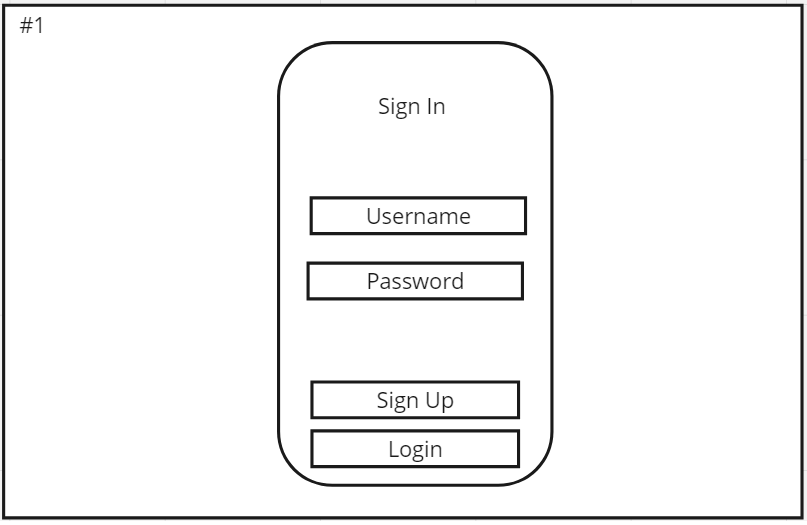
\includegraphics[width=12cm]{Images/login.png}
    \caption{Login Page}
    \label{fig:login}
\end{figure}
\begin{figure}[H]
    \centering
    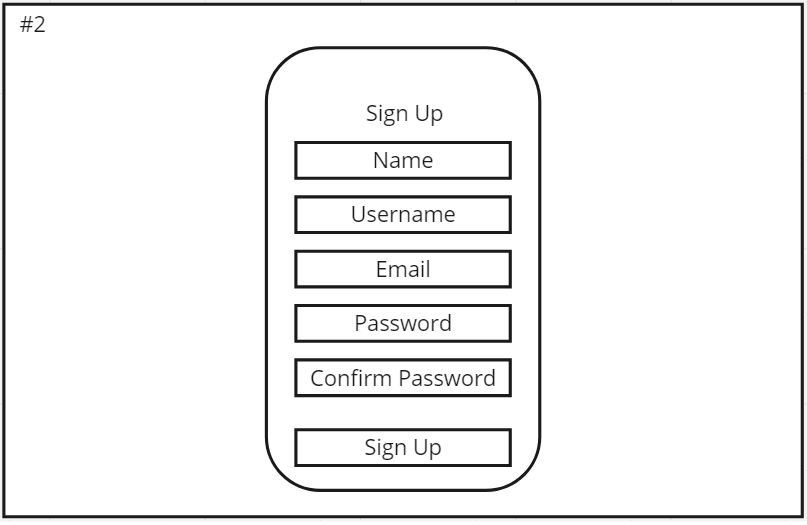
\includegraphics[width=12cm]{Images/signup.png}
    \caption{Sign Up Page}
    \label{fig:signup}
\end{figure}
\begin{figure}[H]
    \centering
    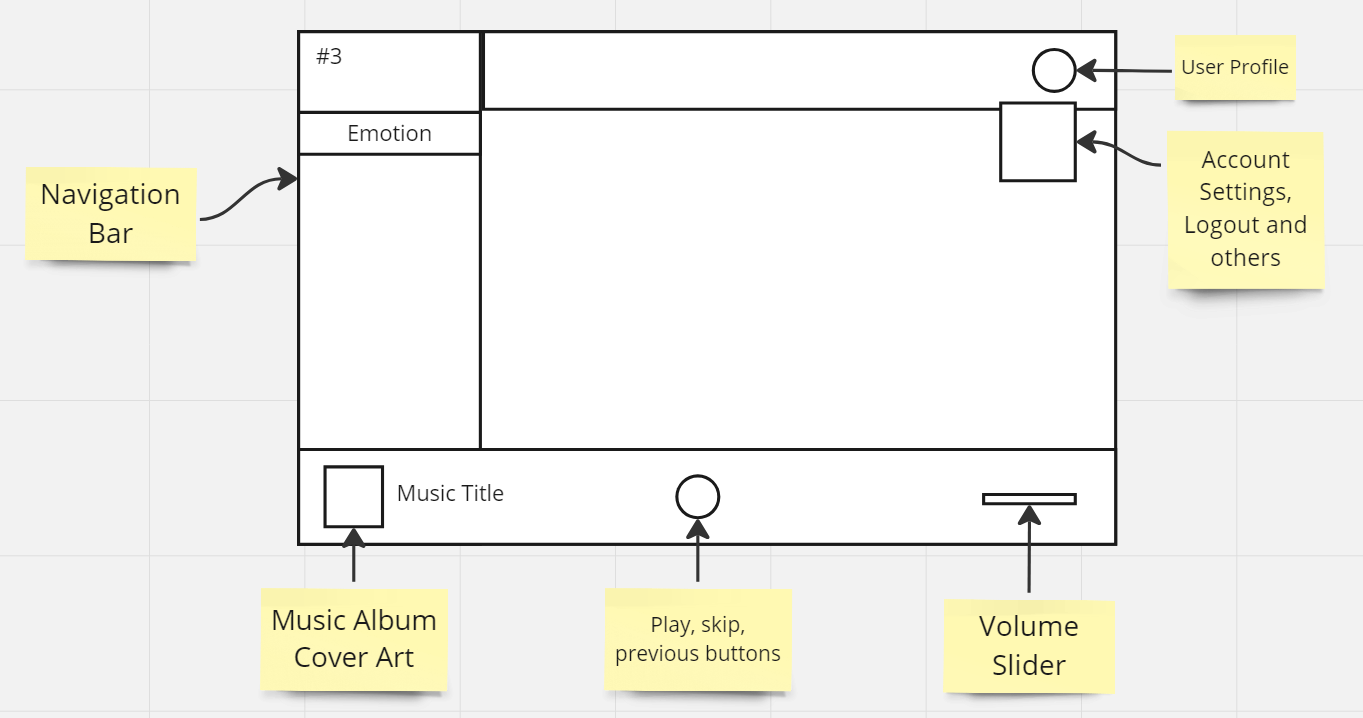
\includegraphics[width=12cm]{Images/overview.png}
    \caption{Dashboard Page}
    \label{fig:dashboard}
\end{figure}
\begin{figure}[H]
    \centering
    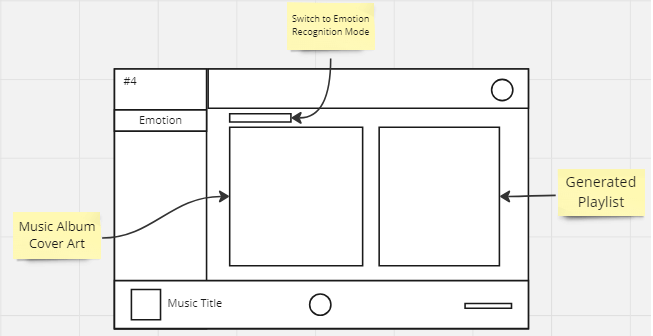
\includegraphics[width=12cm]{Images/emotion.png}
    \caption{Emotion Music Page}
    \label{fig:emotion}
\end{figure}
\begin{figure}[H]
    \centering
    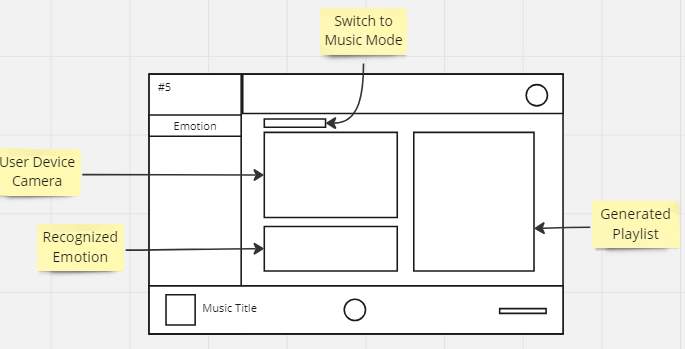
\includegraphics[width=12cm]{Images/detection.png}
    \caption{Emotion Recognition Page}
    \label{fig:emotion-recog}
\end{figure}
\begin{figure}[H]
    \centering
    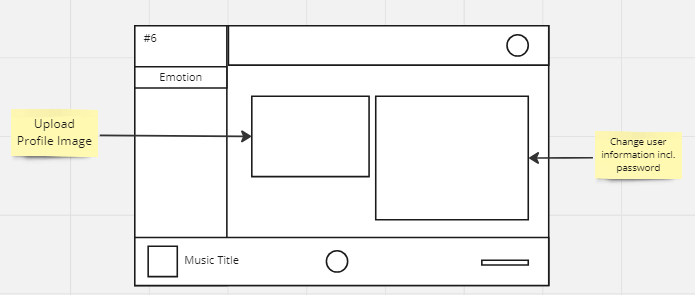
\includegraphics[width=12cm]{Images/user-settings.png}
    \caption{User Settings Page}
    \label{fig:usr-settings}
\end{figure}

\section{Artificial Intelligence and Machine Learning}
\subsection{Models Architecture}
In computer vision, a model's architecture is the basis that backs up its capacity for learning and generalization.
The design decisions made when structuring a model determine not only its performance, but also its efficiency in extracting and understanding the complex patterns found in the data. 
A \gls{fer} model must be able to manage the complexity of human facial emotions with ease. 
Therefore, the architectures explored and selected are designed with the goal of capturing a complex hierarchy of features.
\begin{table}[h!]
    \centering
    \begin{tabular}{>{\ttfamily}l>{\ttfamily}l>{\ttfamily}r}
        \toprule 
        \textbf{Layer (Type)} & \textbf{Output Shape} & \textbf{Parameters} \\
        \midrule
        Input & (None, 48, 48, 1) & 0 \\ 
        Conv2D (3x3x32) & (None, 48, 48, 32) & 320 \\
        Conv2D (3x3x64) & (None, 48, 48, 64) &  18,496\\
        BatchNormalization & (None, 48, 48, 64) & 256 \\
        MaxPooling2D (2x2) & (None, 24, 24, 64) & 0 \\
        Dropout & (None, 24, 24, 64) & 0 \\
        Conv2D (3x3x128) & (None, 24, 24, 128) & 73,856 \\
        Conv2D (3x3x256) & (None, 22, 22, 256) &  295,168\\
        BatchNormalization & (None, 22, 22, 256) & 1,024 \\
        MaxPooling2D (2x2) & (None, 11, 11, 256) & 0 \\
        Dropout & (None, 11, 11, 256) & 0 \\
        Flatten & (None, 30976) & 0 \\
        Dense & (None, 1024) & 31,720,448 \\
        Dropout & (None, 1024) & 0 \\
        Dense (Softmax) & (None, 4) & 4,100 \\
        \bottomrule 
    \end{tabular}
    \caption{Detailed Architecture of the CNNs Model 1}
    \label{tab:cnn-model-1}
\end{table}
\\
\indent Model 1 (Table \ref{tab:cnn-model-1}) is the first attempt at tackling the challenging issue of \gls{fer}, based on the well-proven architectures similar to VGG-16 \citep{simonyan2015deep}, which are intended to identify nad leverage the strengths of facial feature differentiation.
The model started with a conservative number of filters in the \gls{conv2d}, from 32 and incrementally increasing to 64, 128, and 256, to ensure the model is able to capture a spectrum of features from basic to complex. 
Those interspersed `Dropout' layers are used to prevent over-fitting, which then giving the model greater generalization capabilities.
\\
\indent In order to reduce dimensionality, pooling layers are implemented throughout the architecture.
This will compress the spatial volume of features before they are flattened into a format suitable for dense network processing.
The learning process ends in the `Dense' layers that, through a `Softmax' activation, control the emotional categorization, converting the complex network of extracted features into perceptible emotional states.
\begin{table}[h!]
    \centering
    \begin{tabular}{>{\ttfamily}l>{\ttfamily}l>{\ttfamily}r}
        \toprule 
        \textbf{Layer (Type)} & \textbf{Output Shape} & \textbf{Parameters} \\
        \midrule 
        Input & (None, 48, 48, 1) & 0 \\
        Conv2D (3x3x64) & (None, 48, 48, 64) & 640 \\
        BatchNormalization & (None, 48, 48, 64) & 256 \\
        ReLU Activation & (None, 48, 48, 64) & 0 \\
        Conv2D (3x3x64) & (None, 48, 48, 64) & 36,928 \\
        BatchNormalization & (None, 48, 48, 64) & 256 \\
        ReLU Activation & (None, 48, 48, 64) & 0 \\
        MaxPooling2D (2x2, stride 2) & (None, 24, 24, 64) & 0 \\
        Conv2D (3x3x128) & (None, 24, 24, 128) & 73,856 \\
        BatchNormalization & (None, 24, 24, 128) & 512 \\
        ReLU Activation & (None, 24, 24, 128) & 0 \\
        Conv2D (3x3x128) & (None, 24, 24, 128) & 147,584 \\
        BatchNormalization & (None, 24, 24, 128) & 512 \\
        ReLU Activation & (None, 24, 24, 128) & 0 \\
        MaxPooling2D (2x2, stride 2) & (None, 12, 12, 128) & 0 \\
        Conv2D (3x3x256) & (None, 12, 12, 256) & 295,168 \\
        BatchNormalization & (None, 12, 12, 256) & 1,024 \\
        ReLU Activation & (None, 12, 12, 256) & 0 \\
        Conv2D (3x3x256) & (None, 12, 12, 256) & 590,080 \\
        BatchNormalization & (None, 12, 12, 256) & 1,024 \\
        ReLU Activation & (None, 12, 12, 256) & 0 \\
        Conv2D (3x3x256) & (None, 12, 12, 256) & 590,080 \\
        BatchNormalization & (None, 12, 12, 256) & 1,024 \\
        ReLU Activation & (None, 12, 12, 256) & 0 \\
        MaxPooling2D (2x2, stride 2) & (None, 6, 6, 256) & 0 \\
        Flatten & (None, 9216) & 0 \\
        Dense & (None, 4096) & 37,752,832 \\
        BatchNormalization & (None, 4096) & 16,384 \\
        ReLU Activation & (None, 4096) & 0 \\
        Dense & (None, 4096) & 16,781,312 \\
        BatchNormalization & (None, 4096) & 16,384 \\
        ReLU Activation & (None, 4096) & 0 \\
        Dense (Softmax) & (None, 4) & 16,388 \\ 
        \bottomrule 
    \end{tabular}
    \caption{Detailed Architecture of the CNNs Model 2}
    \label{tab:cnn-model-2}
\end{table}
\\
\indent Model 2 (Table \ref{tab:cnn-model-2}) is a refined version of the \gls{fer} model.
With the addition of L2 regularization and a varied number of filter sizes, this model differs from the first model.
This version provides theoretical performance improvements, such as higher generalization in unseen data.
Additionally, this model version is more similar to the VGG-16 model; but, because of resource constraints, the original VGG-16 model, which in theory should yield better results, is not implemented in order to use fewer computer resources.
   
    
    